\documentclass[10pt]{beamer}
\usepackage{amsmath}
\usepackage{amssymb}
%\usepackage{dsfont}
\usepackage{accents}
\usepackage{hyphenat}
\usepackage{multirow}
\usepackage{animate}
\usetheme[progressbar=frametitle]{metropolis}
\setbeamercolor{background canvas}{bg=white}
% \usetheme{focus}
\usepackage{appendixnumberbeamer}
\usefonttheme[onlymath]{serif}
\usepackage{booktabs}
\usepackage[scale=2]{ccicons}

\usepackage{pgfplots}
\usepgfplotslibrary{dateplot}

\usepackage{xspace}
\newcommand{\themename}{\textbf{\textsc{metropolis}}\xspace}
\usetikzlibrary{snakes,arrows,mindmap,trees,backgrounds,shapes.geometric,calc}
\tikzset{graphics/.style={inner sep=0,outer sep=0}}
\tikzset{scaleall/.style={scale=#1, transform shape}}
\usepgflibrary{arrows}


\newlength{\bbw}
\newlength{\bbh}
\newcommand{\pcuad}[3][]{
  % First arguments is an optional prefix for the coordinate names

  \setlength{\bbw}{#2}
  \setlength{\bbh}{#3}
  \useasboundingbox(0,0) rectangle (\bbw,\bbh);

  \path(.5\bbw,.5\bbh) coordinate(#1cp);
  \path(\bbw,0)        coordinate(#1se);
  \path(0,0)           coordinate(#1sw);
  \path(0,\bbh)        coordinate(#1nw);
  \path(\bbw,\bbh)     coordinate(#1ne);
 
  
  \path(\bbw,.5\bbh) coordinate(#1ep);
  \path(.5\bbw,0)    coordinate(#1sp);
  \path(.5\bbw,\bbh) coordinate(#1np);
  \path(0,.5\bbh)    coordinate(#1wp);
       
  \path(.75\bbw,.5\bbh) coordinate(#1hr);
  \path(.25\bbw,.5\bbh) coordinate(#1hl);
  \path(.5\bbw,.25\bbh) coordinate(#1vl);
  \path(.5\bbw,.75\bbh) coordinate(#1vu);

  \path(.75\bbw,.75\bbh) coordinate(#1c1);
  \path(.25\bbw,.75\bbh) coordinate(#1c2);
  \path(.25\bbw,.25\bbh) coordinate(#1c3);
  \path(.75\bbw,.25\bbh) coordinate(#1c4);


%  +-----------------------------------------------+
%  |nw                    np                     ne|
%  |                                               |
%  |                                               |
%  |          c2          vu          c1           |
%  |                                               |
%  |                                               |
%  |wp        hl          cp          hr         ep|
%  |                                               |
%  |                                               |
%  |          c3          vl          c4           |
%  |                                               |
%  |                                               |
%  |sw                    sp                     se|
%  +-----------------------------------------------+
}
 
        
\newcommand{\showcuad}[1][]{

   \draw[help lines,xstep=.5,ystep=.5,gray!10] (#1sw) grid (#1ne);
   \draw[help lines,xstep=1,ystep=1,gray]      (#1sw) grid (#1ne);
   %\draw[help lines,xstep=.25,ystep=.25,gray!20] (sw) grid (ne);
   % \draw[help lines,xstep=1,ystep=1,gray] (sw) grid (ne);
   % \foreach \x in {-20,-14.5,...,20} {
   %     \node [anchor=north, gray,yshift=30] at (\x,0) {\tiny \bf \x};
   %     \node [anchor=east,gray,xshift=30] at (0,\x) {\tiny \bf  \x};
   % }
               
    \fill(#1se) circle(.1) node[anchor=south east]{#1se};
    \fill(#1sw) circle(.1) node[anchor=south west]{#1sw};
    \fill(#1ne) circle(.1) node[anchor=north east]{#1ne};
    \fill(#1nw) circle(.1) node[anchor=north west]{#1nw};
                  
    \fill(#1hr) circle(.1) node[above]{#1hr};
    \fill(#1hl) circle(.1) node[above]{#1hl};
    \fill(#1vu) circle(.1) node[above]{#1vu};
    \fill(#1vl) circle(.1) node[above]{#1vl};
                  
    \fill(#1sp) circle(.1) node[anchor=south]{#1sp};
    \fill(#1wp) circle(.1) node[anchor=west] {#1wp};
    \fill(#1np) circle(.1) node[anchor=north]{#1np};
    \fill(#1ep) circle(.1) node[anchor=east] {#1ep};

    \fill(#1cp) circle(.1) node[above]{#1cp};
    \fill(#1c1) circle(.1) node[above]{#1c1};
    \fill(#1c2) circle(.1) node[above]{#1c2};
    \fill(#1c3) circle(.1) node[above]{#1c3}; 
    \fill(#1c4) circle(.1) node[above]{#1c4};

    %\fill[red](cp|-c1) circle(.1) node[anchor=north]{cp|-c1};

}

\newcommand{\ds}{\displaystyle}
\newcommand{\dsum}{\displaystyle \sum}
\newcommand{\uu}[1]{{\boldsymbol #1}}
\newcommand{\ud}{\,\mathrm{d}}
\def\ttau{\uu{\tau}}
\def\bb{\uu{b}}
\def\nb{\uu{n}}
\def\pb{\uu{p}}
\def\wb{\uu{w}}
\def\xb{\uu{x}}
\def\ab{\uu{a}}
\def\mb{\uu{m}}
\def\yb{\uu{y}}
\def\vb{\uu{v}}
\def\fb{\uu{f}}
\def\zb{\uu{z}}
\def\Xb{\uu{X}}
\def\etab{\uu{\eta}}
\def\thetab{\uu{\theta}}
\def\lambdab{\uu{\lambda}}
\def\gammab{\uu{\gamma}}
\def\taub{\uu{\tau}}
\def\varphib{\uu{\varphi}}
\def\Ab{\uu{A}}
\def\Bb{\uu{B}}
\def\Gb{\uu{G}}
\def\Fb{\uu{F}}
\def\Jb{\uu{J}}
\def\Rb{\uu{R}}
\def\Tb{\uu{T}}
\def\rb{\uu{r}}
\def\ab{\uu{a}}
\newcommand{\molar}[1]{\underaccent{\bar}{#1}}
\def\um{\molar{U}}
\def\hm{\molar{H}}
\def\sm{\molar{S}}
\def\am{\molar{A}}
\def\gm{\molar{G}}
\def\hh{\hat{H}}
\def\sh{\hat{S}}
\def\vm{\molar{V}}
\def\cp{C_{\rm P}}
\def\cv{C_{\rm V}}
\def\cps{C_{\rm P}^*}
\def\cvs{C_{\rm V}^*}
\def\wsd{\dot{W}_s}
\def\md{\dot{M}}\newcommand{\pd}[2]{\left(\frac{\partial {#1}}{\partial 
{#2}}\right)}
\newcommand{\tpd}[3]{\left(\frac{\partial {#1}}{\partial {#2}}\right)_{#3}}
\newcommand{\tpdn}[4]{\left(\frac{\partial^{#4} {#1}}{\partial 
{#2}^{#4}}\right)_{#3}}



\title{Recent simulation methods for resolving molecular details in thermodynamics and kinetics}
\date{October 10, 2019}
\author{Cameron F. Abrams}
\institute{Drexel University, Department of Chemical and Biological Engineering}
\titlegraphic{\hfill
\includegraphics[height=0.75cm]{drexel-horz-blue.png}}

\begin{document}

\maketitle

\begin{frame}{Outline}
  \setbeamertemplate{section in toc}[sections numbered]
  \tableofcontents[hideallsubsections]
\end{frame}

\begin{frame}{Drexel Chemical and Biological Engineering Key Facts}
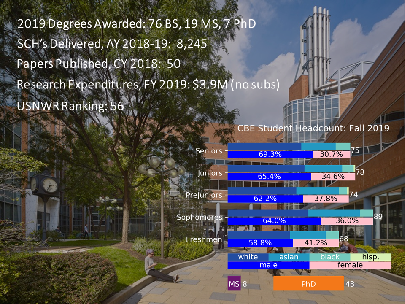
\includegraphics[width=\textwidth]{cbefacts2.pdf}
\end{frame}

\begin{frame}{Drexel Chemical and Biological Engineering Faculty}
\includegraphics[width=\textwidth]{CBEFacultyMugs2019-2.pdf}
\end{frame}

\section{Introduction and Motivation}

\input{motiv1}

\input{essential_problem}

\begin{frame}{Hetergeneous Multiscale Molecular Dynamics (HMMD)}
\begin{tikzpicture}[scaleall=1.0]
\pcuad{\textwidth}{\textheight}
\path(nw) ++(-1,-0.5) node(graphic1)[anchor=north west]{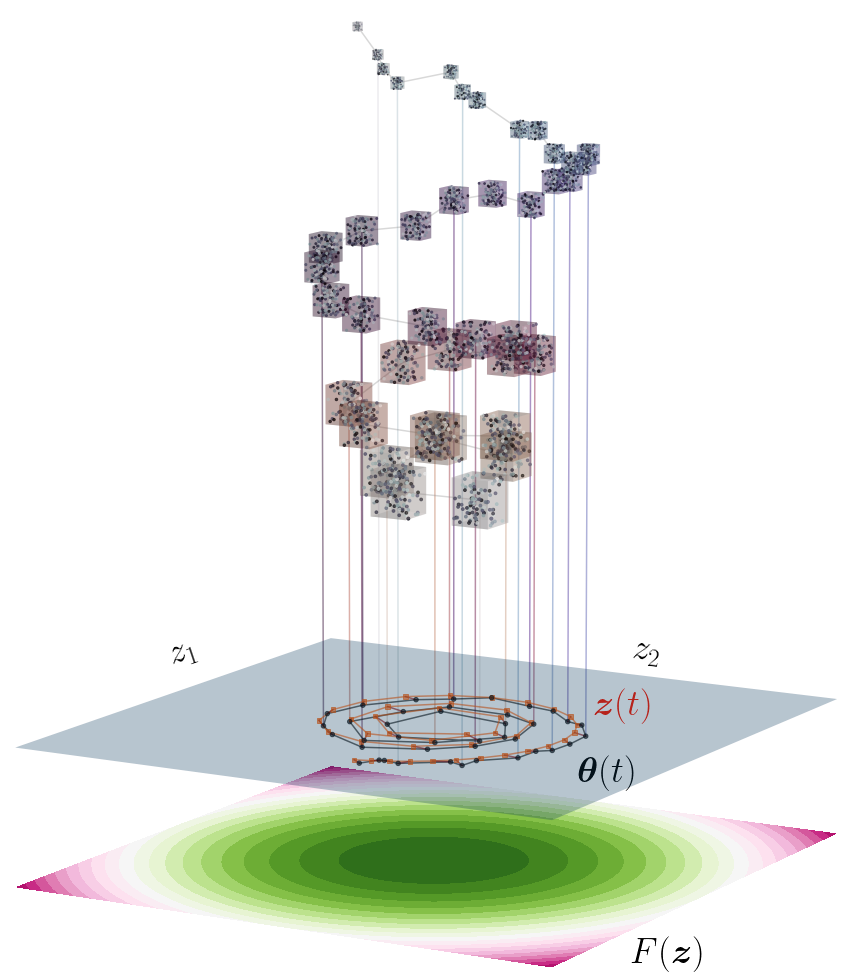
\includegraphics[width=0.6\textwidth]{../hmmdfig2-crop.png}};
\path(np) ++(-1.5,-1) node(line1)[anchor=north west]{Extended configuration space $(\xb^{3N},\ \color{orange!70!black}{\zb^M}\color{black})$}
++(0,-1.5) node(line2)[anchor=west]{$\displaystyle m_i\ddot{x}_i = -\nabla_iV(\xb)-\sum_{j=1}^M\color{green!80!black}{\kappa[\theta_j(\xb)-z_j]}\color{black}\frac{\partial\theta_j}{\partial x_i} + \mbox{e.f.}$}
++(0,-1) node(line3)[anchor=west]{$\displaystyle\bar{m}_j\ddot{z}_j = \sum_{k=1}^{M} \mathcal{M}_{jk}\color{green!80!black}{\kappa[\theta_k(\xb)-z_k]}\color{black} + \color{blue!80!black}{\mbox{bias}}\color{black}$}
++(1,-1.2) node(line4)[anchor=west,align=left] {\textcolor{green!80!black}{Forces} link $\xb$ and $\color{orange!70!black}{\zb}\color{black}$}
++(0,-1) node[anchor=west,align=left,text width=0.6\textwidth] {\textcolor{blue!80!black}{Bias} on $\color{orange!80!black}{\zb}\color{black}$ drives sampling of feature space};
%\draw[] (1.25,2) node {$\thetab(\xb)$};
%\draw[] (2.5,1.75) node {$\zb$};
\end{tikzpicture}
\end{frame}


\section{Temperature-Accelerated MD}

\begin{frame}[fragile]{Enhanced-Sampling MD via Collective-Variable Biasing}

Basic idea:  Map $3N$-dimensional configuration space onto a low-dimensional 
``collective variable'' space:
\begin{align*}
\thetab : \mathbb{R}^{3N}\mapsto\mathbb{R}^{M} \ \ \mbox{and}\ \ \ M \ll 3N\ \ \ 
&\Rightarrow\ \ \zb^{M} = \thetab(\xb^{3N})\\
\Rightarrow\ e^{-\beta F(\zb)} = \int d\xb \ 
\delta(\thetab(\xb)-\zb)\ \rho(\xb) & \equiv P(\zb)
\end{align*}
\vspace{-0.5cm}
\begin{itemize}
\item Probability $P(\zb) = e^{-\beta F(\zb)}$:  \textcolor{blue}{\em central objective of 
enhanced sampling};
\item \textcolor{red}{Problem}: Need to bias sampling to transit regions in CV-space with low $P$ (AKA ``free-energy barriers'').
\item \textcolor{green!80!black}{Optimum bias}: $\ds V_b(\xb) = V(\xb) - F[\thetab(\xb)]$:
\begin{displaymath}
\Rightarrow\ \langle X \rangle = \int d\zb\ \langle X\rangle_{\zb}\  P(\zb) = \frac{\langle X e^{\beta F}\rangle_b}{\langle e^{\beta F}\rangle_b}.
\end{displaymath}
%\item $\langle X\rangle_{\zb}$ via {\em restricted sampling};
\item If we have $F(\zb)$, we can sample better, but we need to sample {\em perfectly} already to get $F(\zb)$...
\item \textcolor{blue}{\it What if we can sample better without knowing $F(\zb)$?}
\end{itemize}
\end{frame}

\begin{frame}[fragile]{Temperature-Accelerated MD}
\vspace{-5mm}
\textcolor{blue}{\tiny Maragliano and Vanden-Eijnden, {\it Chem Phys Lett} {\bf 
426}:168 (2006)}

Extended potential energy:\ \ $\displaystyle U(\xb,\zb) = V(\xb) + 
\frac{1}{2}\kappa\sum_{j=1}^{M}[\theta_j(\xb)-z_j]^2]$\\
Dynamics of configurational variables $\xb$ (``restrained MD''):
\begin{displaymath}
m_i\ddot{x}_i = -\frac{\partial V(\xb)}{\partial 
x_i}-\kappa\sum_{j=1}^{M}\left[\theta_j(\xb)-z_j\right]\frac{\partial\theta_j}{
\partial x_i}+\mbox{thermostat @ $\beta$}
\end{displaymath}
Dynamics of auxiliary variables $\zb$ with enforced separation of time-scales:
\begin{displaymath}
\bar\gamma\bar{m}_j\dot{z}_j = \kappa\left[\theta_j(\xb)-z_j\right] + 
(\mbox{noise @ $\bar\beta$}) \approx -\frac{\partial F_{\kappa}}{\partial z_j} + 
\mbox{noise}
\end{displaymath}

$\zb$ responds to free energy like $\xb$ responds to potential energy.\\
Taking $\bar\beta < \beta$ ($\bar{T} > T$)\ $\Rightarrow$\ enhanced sampling in 
a chosen CV-space.

\end{frame}

\begin{frame}[fragile]{Example: TAMD predicts HIV-1 gp120 conformational changes}
\begin{tikzpicture}
\pcuad{\textwidth}{\textheight}
\path(nw) ++(-0.75,0.0) node(text)[anchor=north west,text width=\textwidth]{{\tiny \textcolor{red!80!black}{CFA and E. Vanden-Eijnden {\it PNAS} {\bf 107}:4961 (2010).}}} ++(0,-0.33) node(topfig)[graphics,anchor=north west]{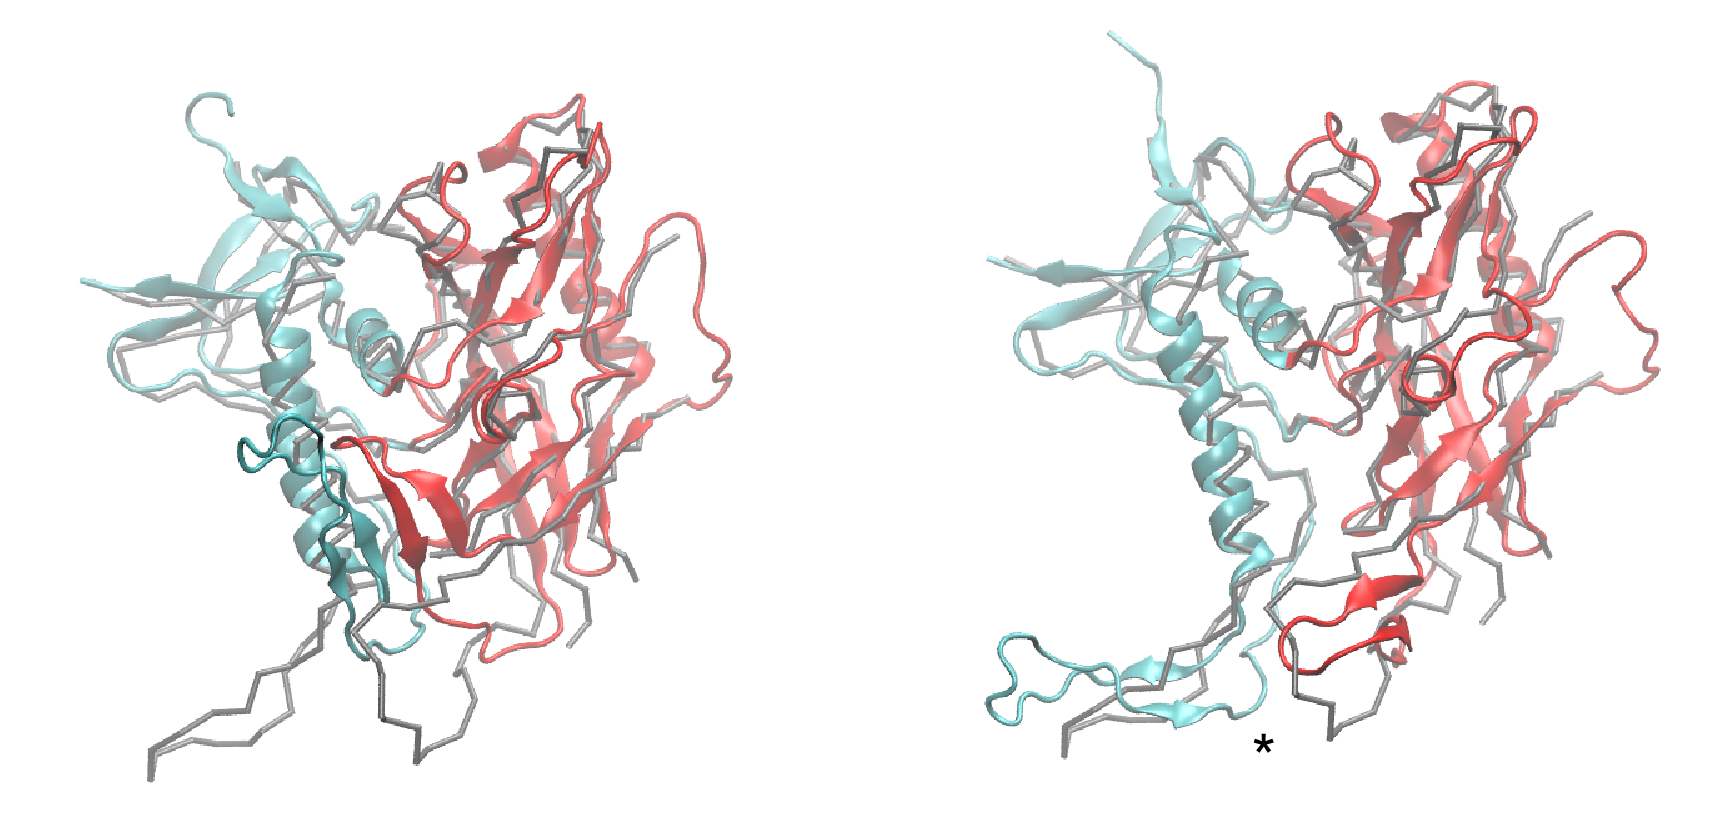
\includegraphics[width=0.8\textwidth]{gp120_snap.png}} ++(0,-4) node(botfig)[graphics,anchor=north west]{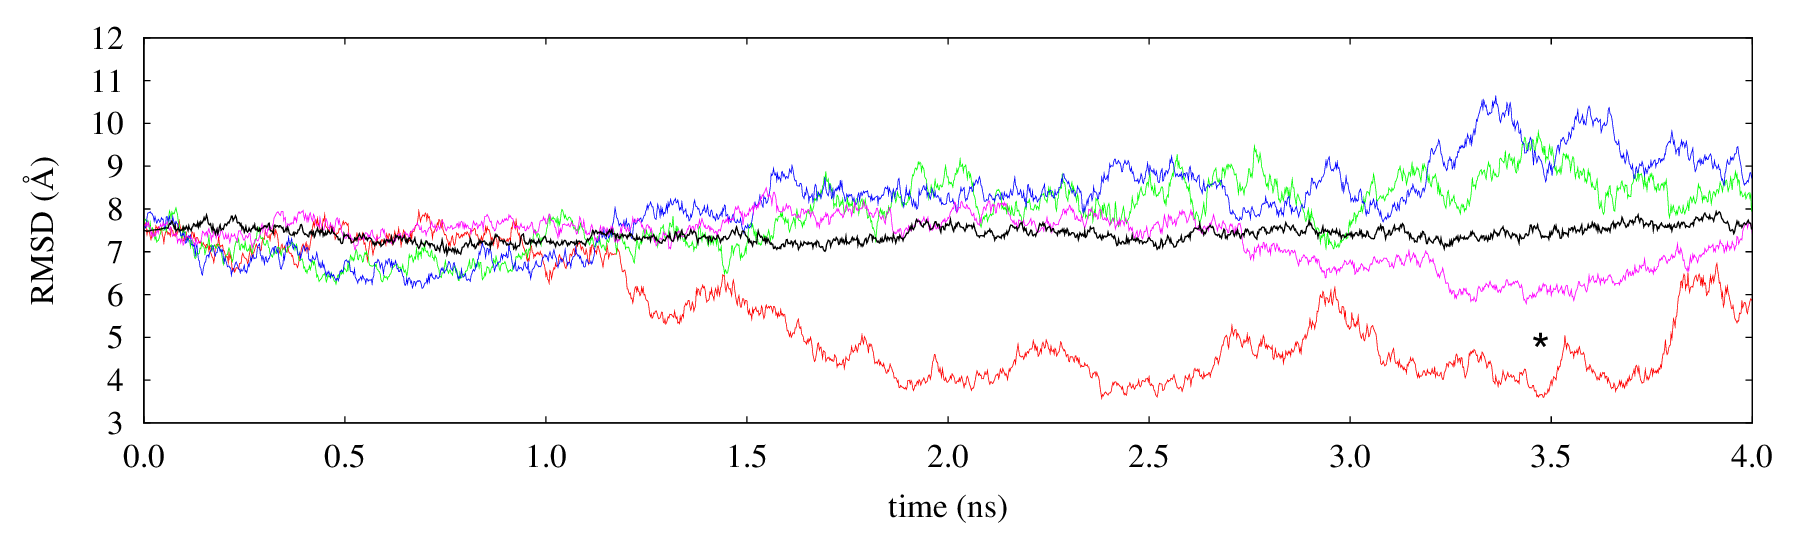
\includegraphics[width=\textwidth]{gp120_rmsdplot.png}}; 
\path(ne) ++(0,0) node(text2)[anchor=north east,text width=0.3\textwidth]{
\begin{itemize}
\item Ribbon: TAMD from 1GC1 (ground state) (\textcolor{teal}{inner}/\textcolor{red}{outer})
\item Tube: Reference from 3HI1 (F105-bound)
\end{itemize}};
\end{tikzpicture}
\end{frame}

\section{The Kv1.2 Channel and 2-D On-the-Fly Parameterization}

\begin{frame}[fragile]{Potassium Channels}
\begin{tikzpicture}[scaleall=1.0]
\pcuad{\textwidth}{\textheight}
%\showcuad
\path(nw) ++(-0.5,0.25) node(corner)[graphics,anchor=north 
west]{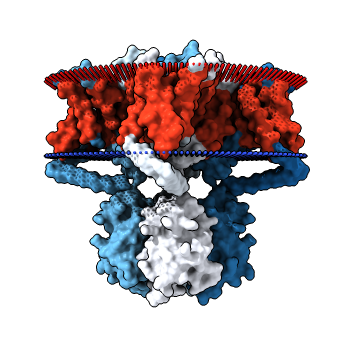
\includegraphics[width=0.33\textwidth]{2a79.png}};
\path(wp) ++(-0.0,1.0) node(corner)[graphics,anchor=north 
west]{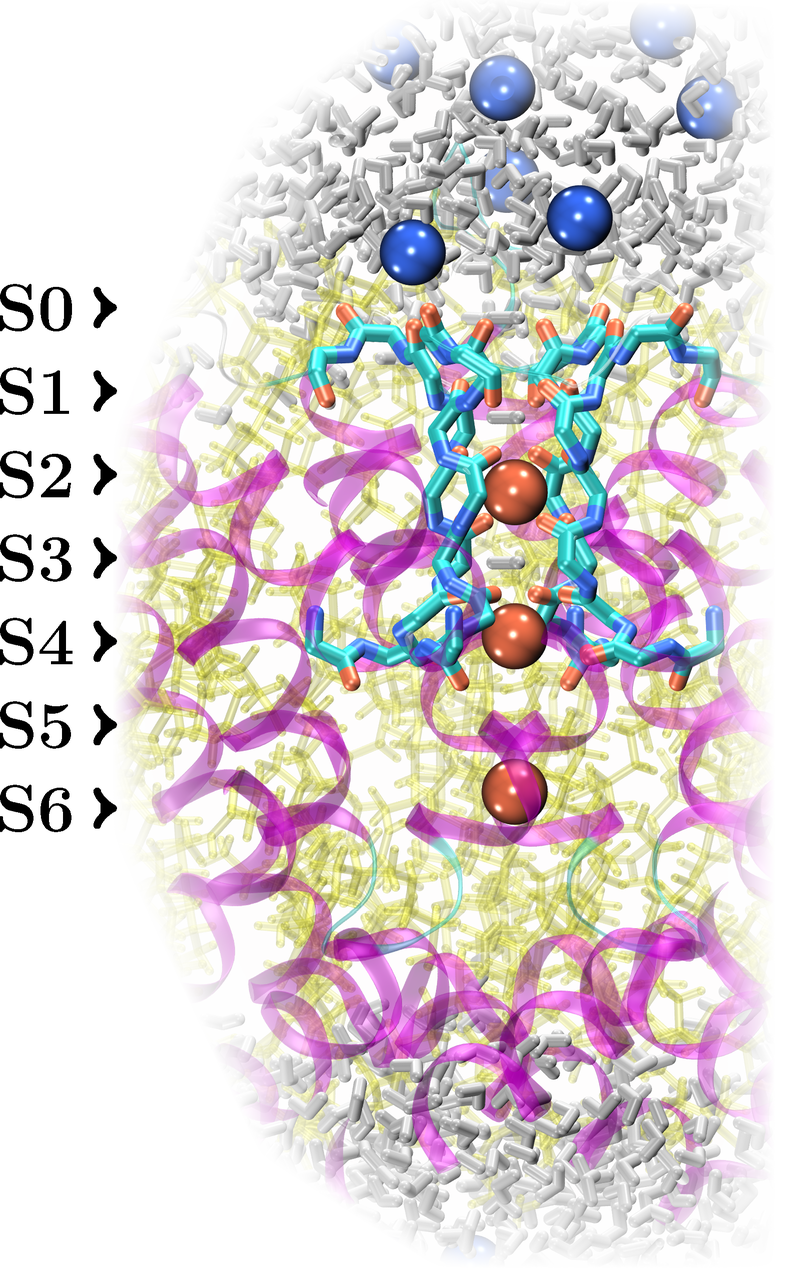
\includegraphics[width=0.25\textwidth]{Kv12_sfilter.png}};
\path(nw) ++(3.5,0) node(text)[anchor=north west,text width=0.65\textwidth]{
\begin{itemize}
\item Responsible for cell membrane {\em depolarization} in action-potential firing
\item Primary function: passive selective transport of K+ ions out of a cell
\item Malfunctioning K channels give rise to ``channelopathies'' like episodic ataxia, neuromyotonia, seizure, and tinnitus
\item Selectivity mechanism is not well-understood because the selectivity filter is complicated
\end{itemize}
};
\end{tikzpicture}

\end{frame}

\begin{frame}{MD Simulation of Kv1.2}
\begin{center}
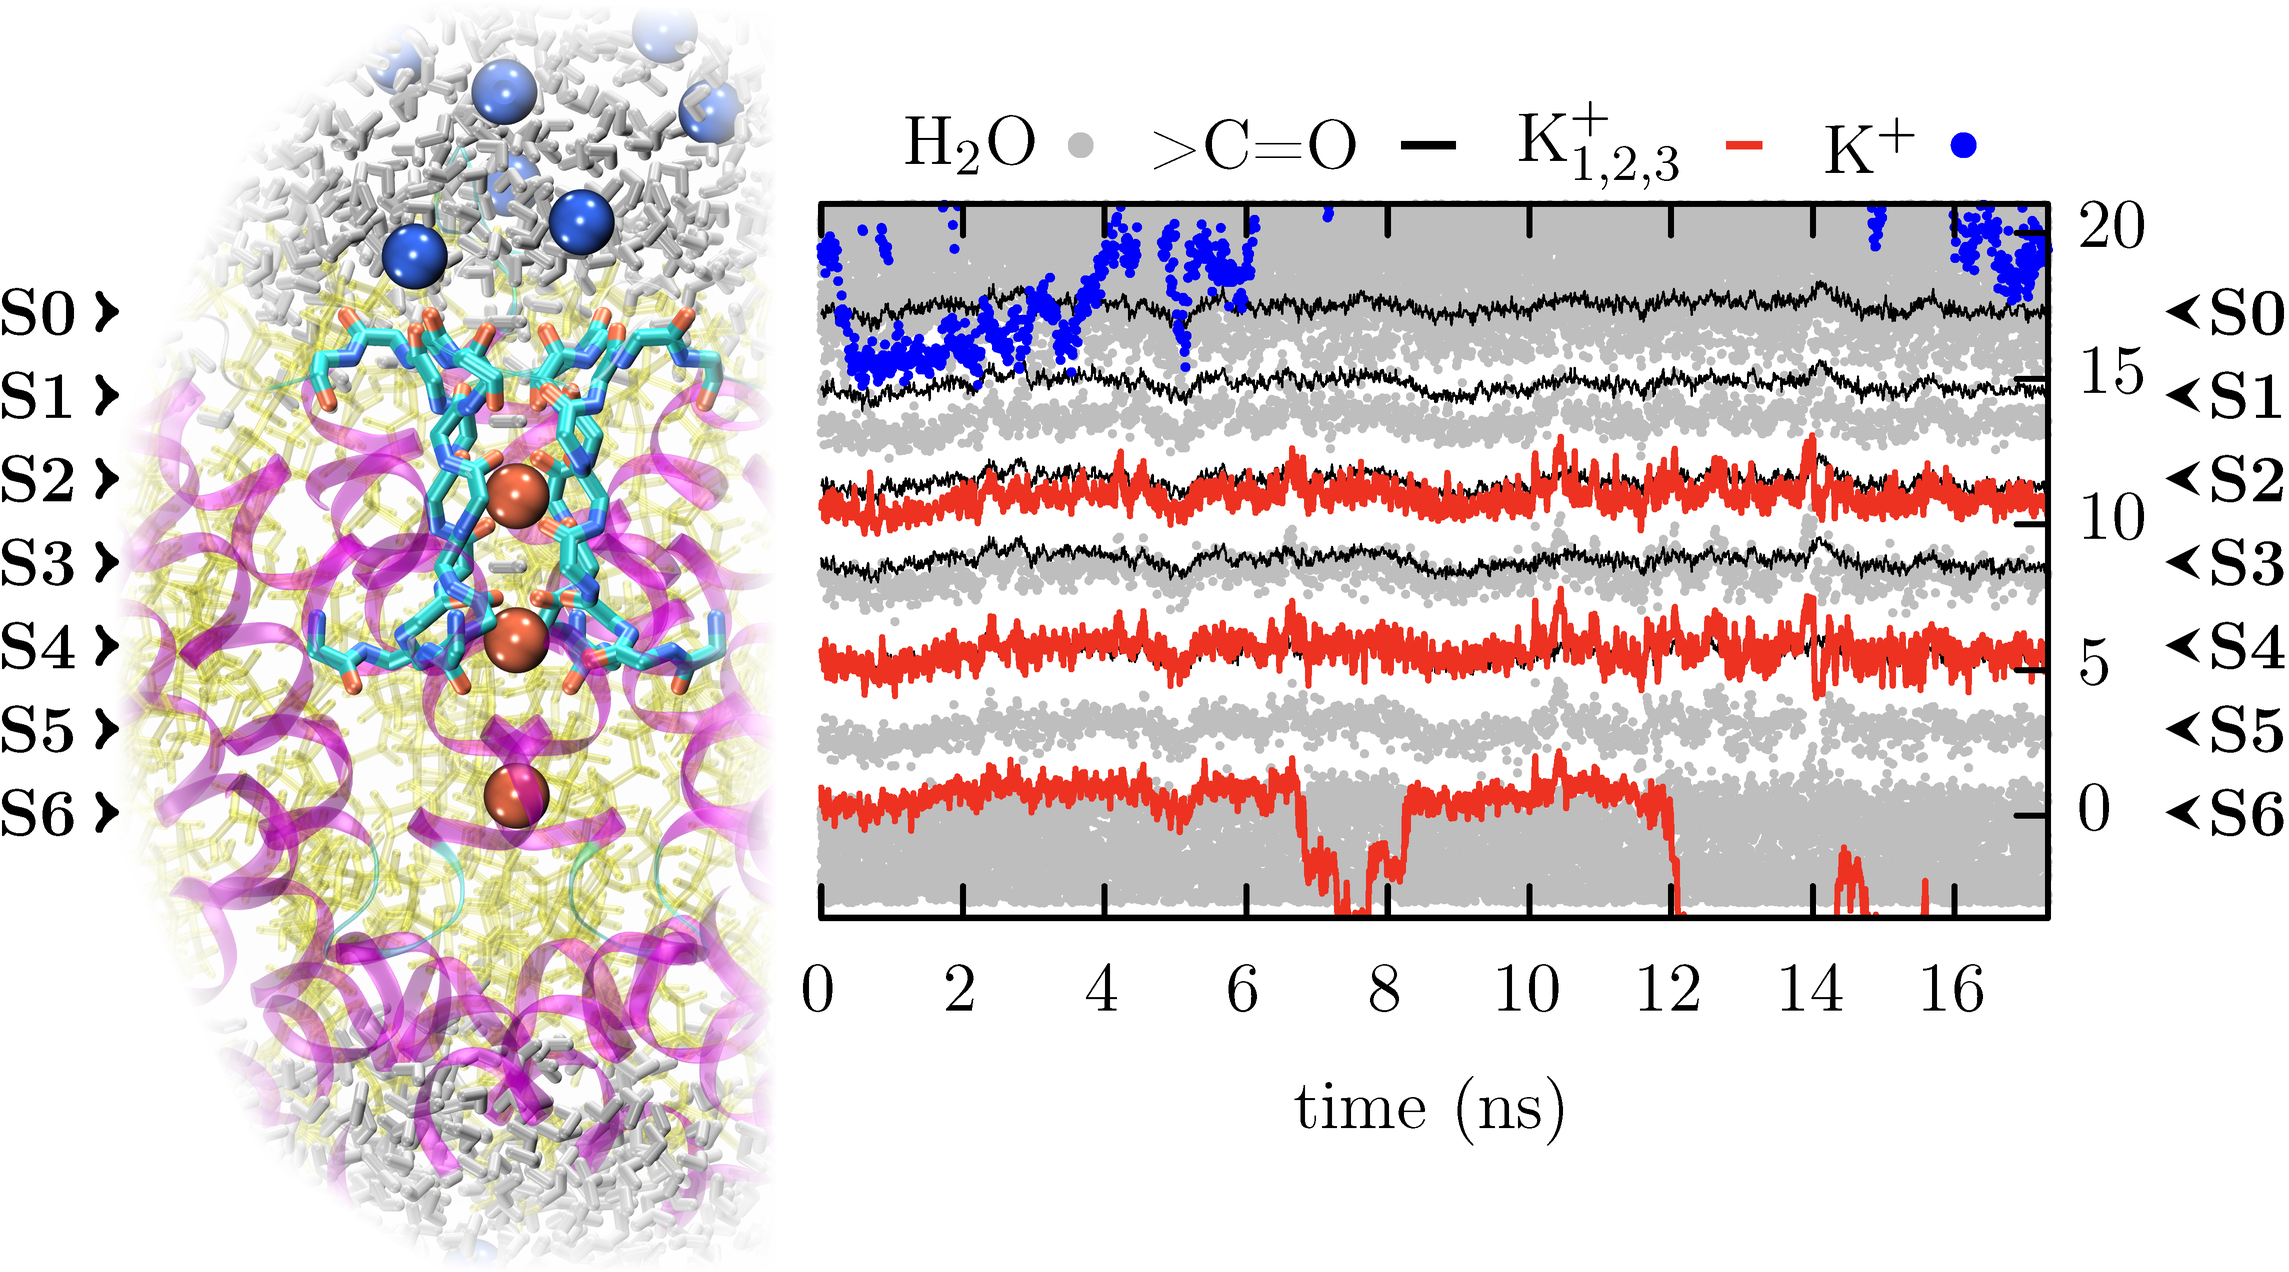
\includegraphics[width=0.75\textwidth]{k12v_md.png}
\end{center}
\begin{itemize}
\item Multi-ion transport with waters supported by 2D-IR and MD\\ {\textcolor{blue}{\small Kratochvil, $\dots$, Roux, $\dots$, Zanni, {\em Science} 2016;{\bf 353}:1040}}.
\item How does water influence free-energy barriers to K$^+$ transport?
\item $z$ coordinate of single ion not enough information:  need higher-dimensional coordinate.
\end{itemize}
\end{frame}

\begin{frame}{2D TAMD Simulation of K$^+$ Transport}
\begin{center}
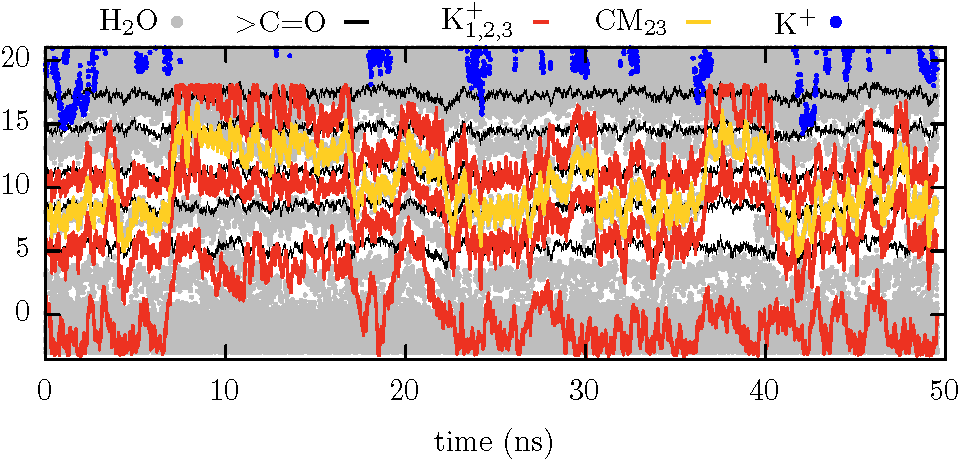
\includegraphics[width=0.9\textwidth]{fullions-crop.png}
\end{center}
\begin{itemize}
\item 2D CV: $z$ of K$_1$ and $z_{\sf CM}$ of (K$_2$,K$_3$)
\item Fictitious temperature 3000 K
\end{itemize}
{\tiny \textcolor{red!80!black}{S. A. Paz, L. Maragliano, and CFA {\em J. Chem. Theory. Comput.} {\bf 14}:2743-2750 (2018)}}
\end{frame} 


\begin{frame}[fragile]{On-the-Fly Free-Energy Parameterization (OTFP)}
\begin{tikzpicture}[scaleall=1.0]
\pcuad{\textwidth}{\textheight}
%\showcuad
\path(nw) ++(-0.75,0.0) node(text)[anchor=north west,text 
width=\textwidth]{{\tiny \textcolor{red!80!black}{CFA and E. Vanden-Eijnden 
{\em Chem Phys Lett} {\bf 547}:114 (2012)}}};
\path(c2) ++(-2.5,1.5) node(text)[anchor=north west,text 
width=\textwidth]{\textcolor{blue}{Basis-function expansion}};
\path(c2) ++(-2.5,1.0) node(text)[anchor=north west,text width=\textwidth]{$\ds 
\tilde{F}(\zb) = \sum_k\lambda_k\phi_k(\zb)$};
\path(c1) ++(-2,1.25) node(text)[anchor=north west,text 
width=\textwidth]{\textcolor{blue}{Error as objective function}};
\path(c1) ++(1,-1) node(text)[anchor=north west,text 
width=\textwidth]{\textcolor{blue}{Minimize}};
\path(c1) ++(1,-1.75) node(text)[anchor=north west,text width=\textwidth]{$\ds 
\frac{\partial E}{\partial \lambdab}=0$};
\path(c1) ++(-3.75,0.75) node(text)[anchor=north west,text 
width=\textwidth]{$\ds E(\lambdab) = \Big< 
\sum_j\left[\kappa[z_j-\theta_j(\xb)]-\frac{\partial \tilde{F}(\zb)}{\partial 
z_j}\right]^2\Big>_{\rm TAMD}$};
\path(cp) ++(1.5,.25) node(text)[anchor=north west,text width=\textwidth]{$\ds 
\uu{A}\lambdab = \uu{b}$};
\path(hl) ++(-2.5,1.25) node(text)[anchor=north west,text width=\textwidth]{$\ds 
A_{nm} = \frac{1}{2}\left<\sum_i\frac{\partial \phi_m(\zb)}{\partial z_i} 
\frac{\partial \phi_n(\zb)}{\partial z_i}\right>_{\rm TAMD}$};
\path(hl) ++(-2.5,-0.25) node(text)[anchor=north west,text 
width=\textwidth]{$\ds b_{m} = \left<\sum_i\frac{\partial \phi_m(\zb)}{\partial 
z_i} \kappa[z_i-\theta_i(\xb)]\right>_{\rm TAMD}$};
\draw[<->,thick,color=green!80!black] (0.1\bbw,0.1\bbh) -- (0.5\bbw,0.1\bbh);
\draw[->,thick,color=green!80!black] (0.3\bbw,0.1\bbh) -- (0.3\bbw,0.25\bbh);
\draw[thick,color=orange!50!black] (0.4\bbw,0.1\bbh) -- (0.3\bbw,0.2\bbh);
\draw[thick,color=orange!50!black] (0.3\bbw,0.2\bbh) -- (0.2\bbw,0.1\bbh);
\draw[thick,color=green!80!black] (0.2\bbw,0.1\bbh) -- (0.2\bbw,0.08\bbh);
\draw[thick,color=green!80!black] (0.4\bbw,0.1\bbh) -- (0.4\bbw,0.08\bbh);
\draw[thick,color=green!80!black] (0.3\bbw,0.1\bbh) -- (0.3\bbw,0.08\bbh);
\draw (0.3\bbw,0.06\bbh) node {$m$};
\draw (0.2\bbw,0.06\bbh) node {$m-1$};
\draw (0.4\bbw,0.06\bbh) node {$m+1$};
\draw (0.32\bbw,0.15\bbh) node {1};
\draw (0.35\bbw,0.25\bbh) node {$\phi_m$};
\draw [->,thick,color=orange!80!black] (0.7\bbw,0.7\bbh) -- (0.85\bbw,0.55\bbh);
\draw [->,thick,color=orange!90!black] (0.85\bbw,0.5\bbh) -- (0.8\bbw,0.5\bbh);
\path(c4) ++(-1.0,1.5) node(text)[anchor=north west,text width=\textwidth]{MD vs OTFP: Butane C$_1$-C$_4$\\ Distance Free Energy};
\path(c4) ++(-1.25,0.65) node(corner)[graphics,anchor=north west]{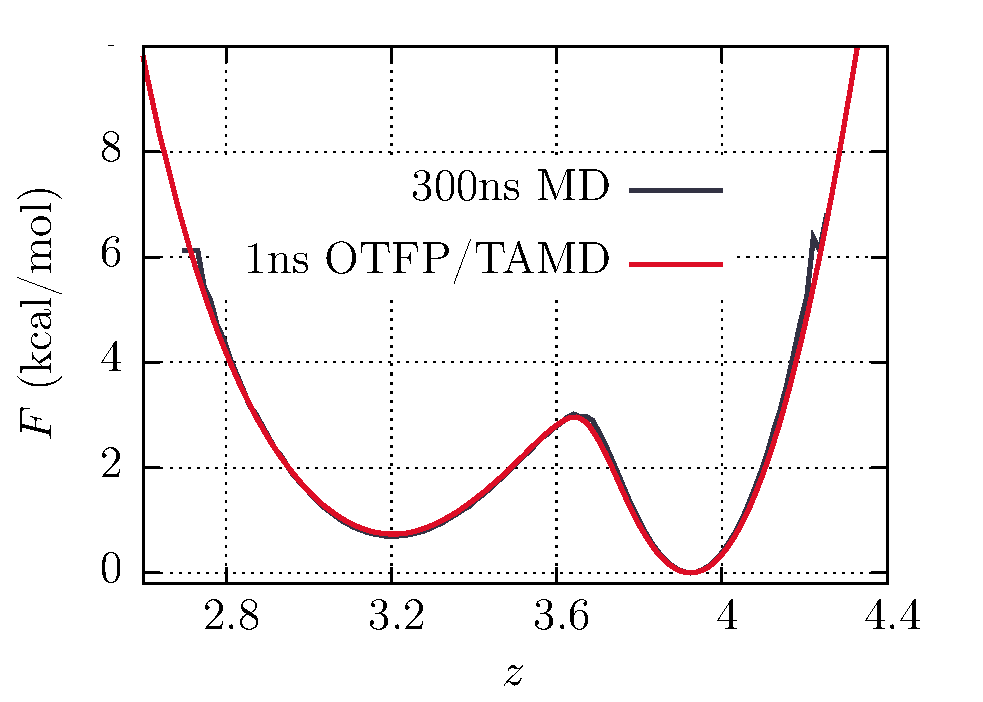
\includegraphics[width=0.33\textwidth]{otfpc4}};
\path(c4) ++(2.25,0.65) node(corner)[graphics,anchor=north west]{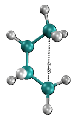
\includegraphics[width=0.1\textwidth]{butane}};
\end{tikzpicture}
\end{frame}

%\section{2D-OTFP and Transport through Ion Channels}

\begin{frame}{From Profiles to Surfaces: Two-Dimensional OTFP}
Two-dimensional chapeaus:
\begin{align*}
\phi_m(z_1,z_2)=
\tilde\phi\left(\dfrac{z_1-z_{1m}}{h_1}+(m-1)\!\!\!\mod N_1,\dfrac{z_2-z_{2m}}{h_2}-\left\lfloor \dfrac{m-1}{N_1}\right\rfloor \right)
\end{align*}
\begin{center}
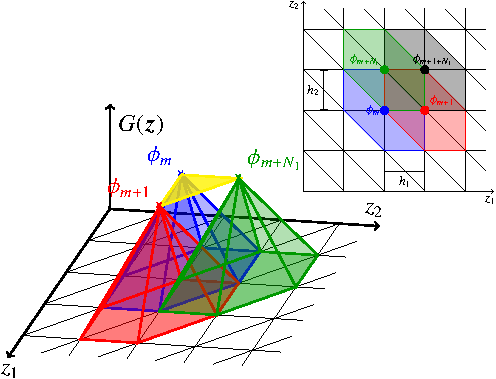
\includegraphics[width=0.65\textwidth]{plane.pdf}
\end{center}
\end{frame}

\begin{frame}{2DOTFP: Validation with Alanine Dipeptide}
\begin{tikzpicture}[scaleall=1.0]
\pcuad{\textwidth}{\textheight}
\path(wp) ++(0.0,0.0) node(aladfig)[anchor=west,text width=0.5\textwidth]{
\includegraphics[width=0.5\textwidth]{aladfig.pdf}};
\path(aladfig) ++(0.5,0.0) node(big)[anchor=west,text width=0.85\textwidth]{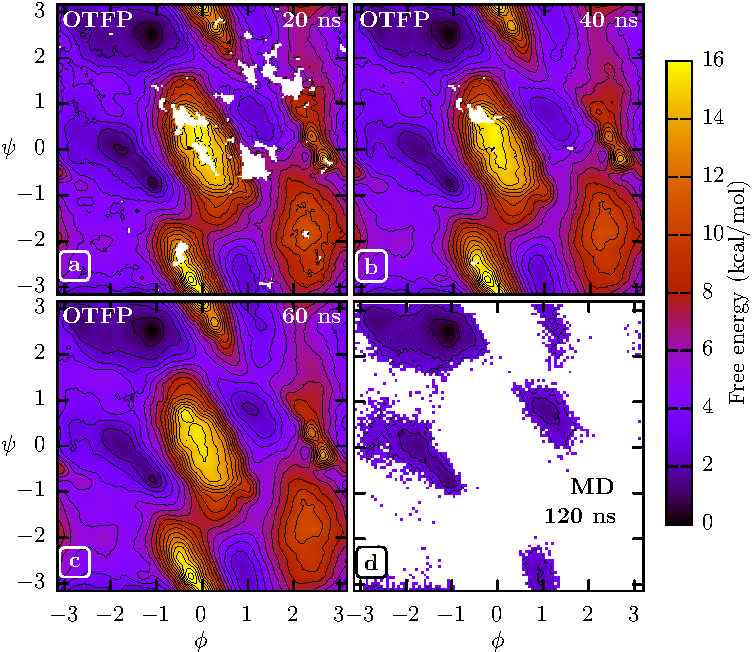
\includegraphics[width=0.85\textwidth]{fesAlad30ns-crop.pdf}};
\end{tikzpicture}
\end{frame}



\begin{frame}{2D OTFP: Transport Minimum Free-Energy Pathways}
\begin{tikzpicture}
\pcuad{\textwidth}{\textheight}
%\showcuad
\path(nw) +(0,0) node(image)[anchor=north west]{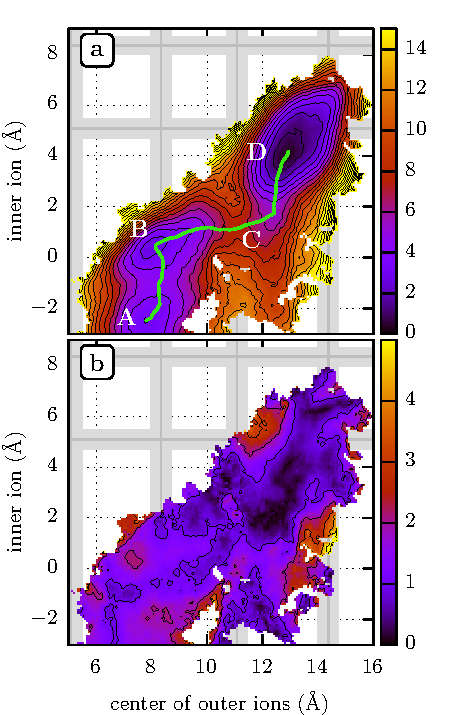
\includegraphics[width=0.5\textwidth]{fullfes_path_err.pdf}};
\path(nw) +(1.5,-4) node(errlab)[anchor=north west]{Error, $N$=3};
\path(nw) +(5,-1.5) node(bullets)[anchor=north west,text width=0.5\textwidth]{\begin{itemize}
\item A$\rightarrow$B: Innermost ion moves up one position
\item B$\rightarrow$C: CM$_{2,3}$ moves up one position, followed quickly by
\item C$\rightarrow$D: Innermost ion moves up one more position
\item $\Rightarrow$ Net translocation of one K$^+$
\item What role is water playing?
\end{itemize}};
\end{tikzpicture}
\end{frame}

\begin{frame}{Water Restraints: Ion-Tethered vs. Excluded-from-Filter}
\begin{tikzpicture}
\pcuad{\textwidth}{\textheight}
%\showcuad
\path(nw) +(0,0) node(image)[anchor=north west]{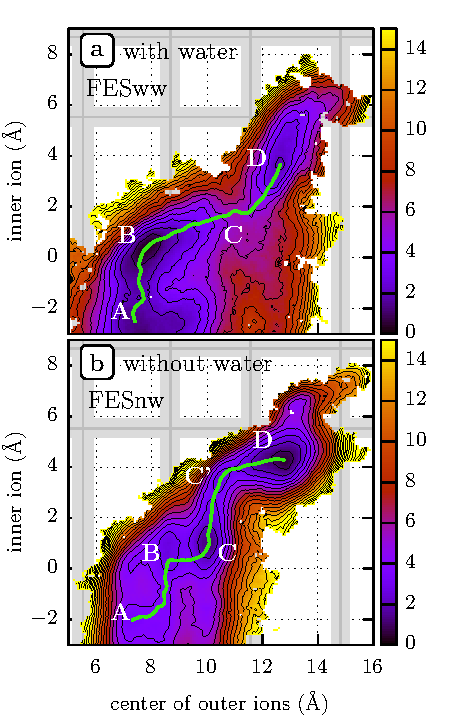
\includegraphics[width=0.5\textwidth]{wc_fes.pdf}};
\path(nw) +(5,-1.5) node(bullets)[anchor=north west,text width=0.5\textwidth]{\begin{itemize}
\item With one water tethered to each K$^+$, FES resembles unrestrained one
\item With water excluded from channel, ion motion is less concerted, more ``hard-knock'' like
\end{itemize}};
\end{tikzpicture}
\end{frame}

\begin{frame}{Free-Energy Profiles along MFEP's}
\begin{tikzpicture}
\pcuad{\textwidth}{\textheight}
%\showcuad
\path(nw) +(0,0.2) node(cite)[anchor=north west]{\tiny \textcolor{red!80!black}{S. A. Paz, L. Maragliano, and CFA {\em J. Chem. Theory. Comput.} {\bf 14}:2743-2750 (2018)}};
\path(np) +(0,0) node(image)[anchor=north]{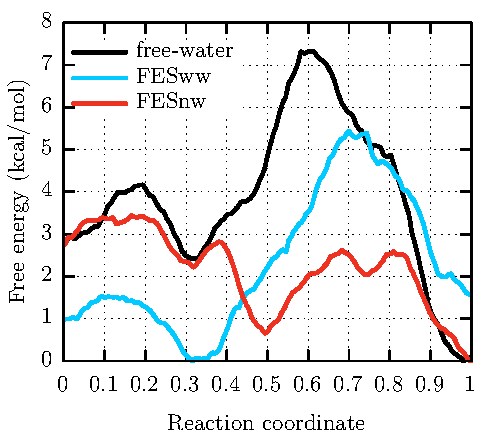
\includegraphics[width=0.67\textwidth]{paths.pdf}};
\path(nw) +(0,-6) node(bullets)[anchor=north west,text width=\textwidth]{\begin{itemize}
\item Energy barriers for unrestricted and ion-tethered water systems are similar; suggests intercalated water is preferred
\item Dry filter shows shallower barriers; dry transport might be faster if water could be actively excluded
\end{itemize}};
\end{tikzpicture}
\end{frame}


\section{Monomeric Sarcosine Oxidase (MSOX) and Markovian Milestoning}

\begin{frame}[fragile]{MSOX:  A Prototypical Flavoenzyme}
\begin{tikzpicture}[scaleall=1.0]
\pcuad{\textwidth}{\textheight}
%\showcuad
\path (nw) ++(0,0) node (heading) [anchor=north west,text width=\textwidth] 
{MSOX is a bacterial enzyme that uses the \textcolor{orange!80!black}{flavin} redox cycle to catalyze oxidative demethylation of sarcosine to glycine.};
\path(c2) ++(0,0.5) node (FoSr) [shape=rectangle,draw] {F$_{\sf O}$S$_{\sf R}$}
          ++(-2,-1.5) node (Fo) [shape=rectangle,draw] {F$_{\sf O}$}
          ++(+2,-1.5) node (Fr) [shape=rectangle,draw] {F$_{\sf R}$}
          ++(+2,1.5) node (FrPo) [shape=rectangle,draw] {F$_{\sf R}$P$_{\sf O}$}
          ++(-2,-3.5) node (FrPoO2) [shape=rectangle,draw] {F$_{\sf R}$P$_{\sf O}$O$_{\sf 2}$};
\path(Fo)  +(0.5,1) node (Sr) [shape=rectangle] {S$_{\sf R}$};
\path(FrPo) +(-1.5,0.0) node (Poa) [shape=rectangle] {P$_{\sf O}$};
\path(FrPo) +(0.0,-2) node (O2a) [shape=rectangle] {O$_{\sf 2}$};
\path(O2a) +(-2.75,0.0) node (O2b) [shape=rectangle] {O$_{\sf 2}$};
\path(Fo) +(1.5,0) node (H2O2a) [shape=rectangle] {H$_{\sf 2}$O$_{\sf 2}$};
\path(Fo) +(-0.5,-1.5) node (Pob) [shape=rectangle] {P$_{\sf O}$};
\path(Pob) +(0,-1) node (H2O2b) [shape=rectangle] {H$_{\sf 2}$O$_{\sf 2}$};
\draw [->,thick] (Fo.north east) -- (FoSr.south west) node(attractor1)[pos=0.90]{};
\draw [->,thick,snake] (FoSr.south east) -- (FrPo);
\draw [->,thick] (FrPo.south west) -- (Fr.north east) node(attractor2)[pos=0.10]{};
\draw [->,thick] (Fr.north west) -- (Fo.south east) node (attractor5)[pos=0.10]{} node(attractor4)[pos=0.70]{};
\draw [->,thick] (FrPo.south) -- (FrPoO2.north east) node(attractor3)[pos=0.60]{};
\draw [->,thick] (FrPoO2.north west) -- (Fo.south) node(attractor6)[pos=0.2]{} node(attractor7)[pos=0.6]{};
\draw [<-,thick] (FoSr.south west) .. controls (attractor1.south west) .. (Sr.east);
\draw [->,thick] (FrPo.south west) .. controls (attractor2.south west) .. (Poa.south east);
\draw [<-,thick,color=red] (FrPoO2.north east) .. controls (attractor3.south) .. (O2a.west);
\draw [->,thick] (Fr.north west) .. controls (attractor4.north west) .. (H2O2a.south west);
\draw [<-,thick,color=blue] (Fo.south east) .. controls (attractor5.north west) .. (O2b.north);
\draw [->,thick] (FrPoO2.north west) .. controls (attractor6.north west) .. (H2O2b.east);
\draw [->,thick] (FrPoO2.north west) .. controls (attractor7.north west) .. (Pob.east);
\path(nw) +(6,-1) node (image) [graphics,anchor=north west] {
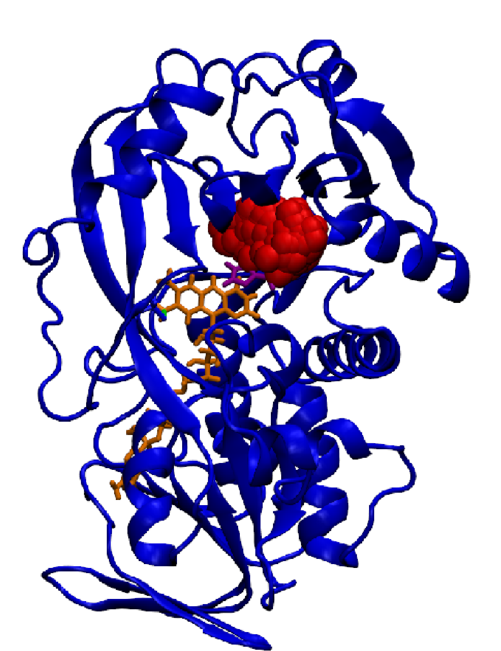
\includegraphics[width=0.45\textwidth]{msox_o2_1}};
\path(c3) +(-2,-0.5) node (sometext) [shape=rectangle,anchor=north west,text width=\textwidth] {
\textcolor{blue}{Ping-pong} vs. \textcolor{red}{Modified ping-pong}};
\end{tikzpicture}
\end{frame}

\begin{frame}[fragile]{Experimental Support for Modified Ping-Pong}
\begin{tikzpicture}[scaleall=1.0]
\pcuad{\textwidth}{\textheight}
%\showcuad
\path(nw) ++(-0.25,-0.4) node(plot)[graphics,anchor=north west]{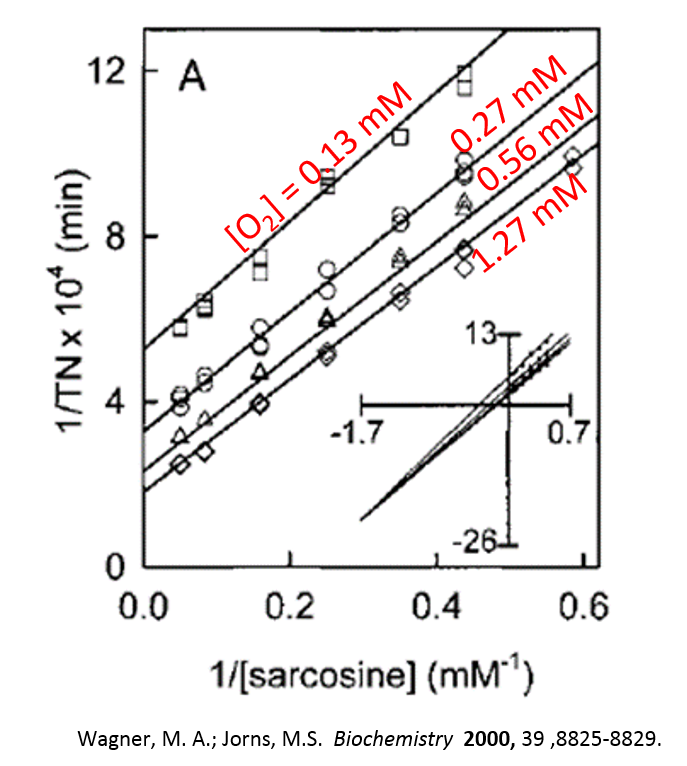
\includegraphics[width=0.6\textwidth]{msox_jorns_expt}}
          ++(6.5,-0.0) node(text) [shape=rectangle,anchor=north west,text width=0.4\textwidth] {
          Lineweaver-Burk slope-dependence on [O$_{\sf 2}$] indicates [O$_{\sf 2}$] and [S$_{\sf R}$] are not independent, suggesting \textcolor{red}{MPP}.}
          ++(0.0,-3.0) node(moretext) [shape=rectangle,anchor=north west,text width=0.4\textwidth]{
          \textcolor{green!80!black}{\bf Hypothesis:} MPP implies kinetics of O$_{\sf 2}$ entry and exit should be 
          sensitive to whether or not substrate is bound.  Test using simulations!};

\end{tikzpicture}
\end{frame}

\begin{frame}[fragile]{Building Up Markovian Milestoning Calculations of Kinetics}
\begin{tikzpicture}[scaleall=1.0]
\pcuad{\textwidth}{\textheight}
%\showcuad
\path(nw) ++(-0.75,0.15) node(text)[anchor=north west,text 
width=\textwidth]{{\tiny \textcolor{red!80!black}{T.-Q. Yu, M. Lapelosa, E. Vanden-Eijnden, and \underline{CFA}
{\em JACS} {\bf 137}:3041 (2015)}}};
\path(nw) ++(-0.5,-1.0) node(moretext)[anchor=north west,text width=0.5\textwidth]{
\begin{itemize}
\item Free energy as a function of ligand location via \textcolor{red}{single-sweep reconstruction}
\item Minimum-free-energy pathways (MFEP's) connecting sites and portals via \textcolor{blue}{string method}
\item Site-to-site and site-to-portal mean first-passage times (MFPT's) for O$_{\sf 2}$ diffusion along MFEP's using \textcolor{green!80!black}{Markovian milestoning}
\end{itemize}};
\path(nw) ++(6,-1) node(image)[anchor=north west]{
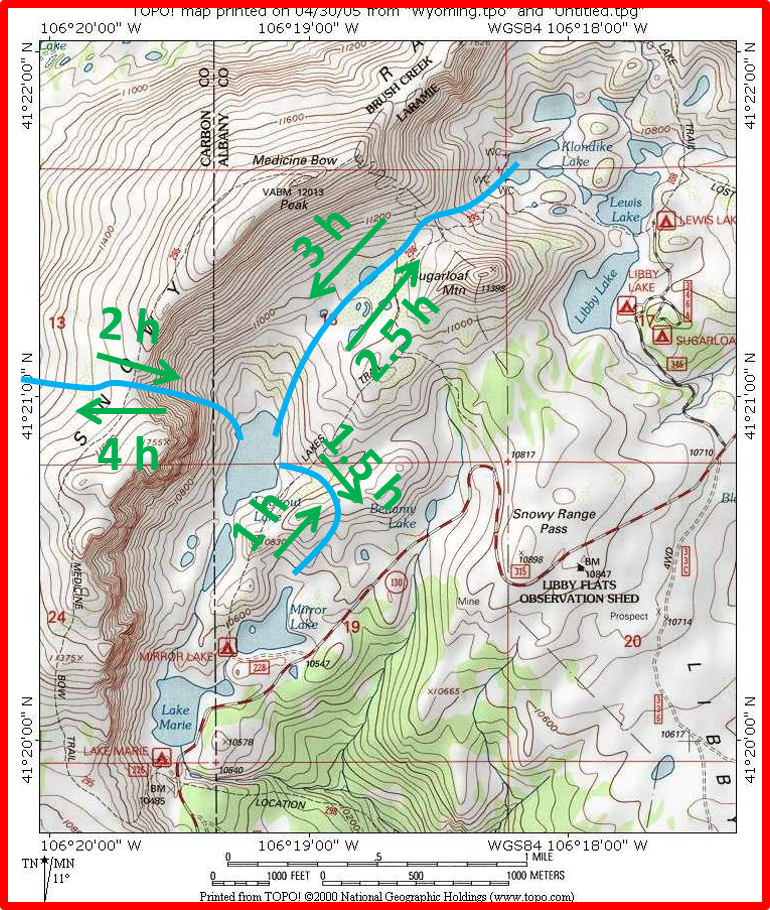
\includegraphics[width=0.5\textwidth]{topo_medicine_bow}};
\end{tikzpicture}
\end{frame}

\begin{frame}[fragile]{Single-Sweep Reconstruction Maps and String-Method Locates Channels}
\begin{tikzpicture}[scaleall=1.0]
\pcuad{\textwidth}{\textheight}
%\showcuad
\path(nw) ++(-0.75,0.15) node(cites)[anchor=north west,text 
width=\textwidth]{{\tiny \textcolor{red!80!black}{
L. Maragliano, G. Cottone, G. Ciccotti, and E. Vanden-Eijnden, {\it JACS} {\bf 312}:1010 (2010)\\
M. Lapelosa and \underline{CFA}, {\it J Chem Theory Comput} {\bf 9}:1265 (2013)\\
A. Bucci and \underline{CFA}, {\it J Chem Theory Comput} {\bf 10}:2668 (2014)\\
}}};
\path(nw) ++(0.0,-0.75) node(cvtext) [anchor=north west,text width=\textwidth] {
$\thetab(\xb)\ :$\ center-of-mass  of O$_{\sf 2}$ in protein-fixed coordinate system.\\
$\Rightarrow$\ $P(\zb)$ = probability of finding O$_{\sf 2}$ at $\zb$ at equilibrium.};
\path(nw) ++(0.0,-2.5) node(pic) [graphics,anchor=north west]{
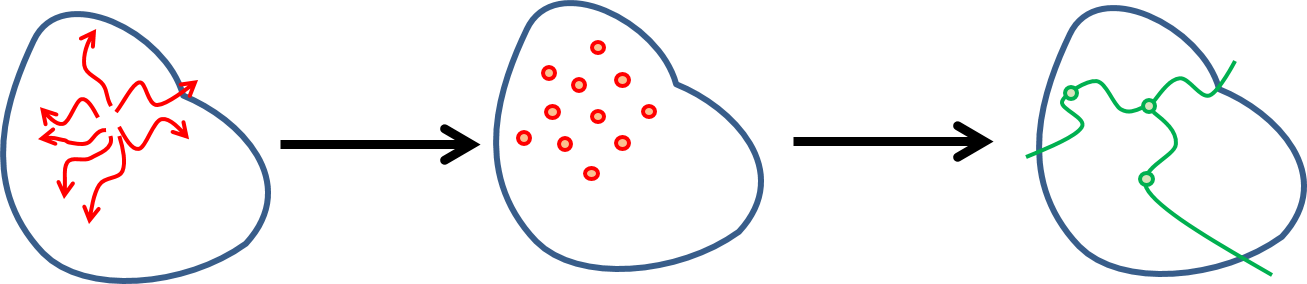
\includegraphics[width=\textwidth]{single_sweep_cartoon}};
\path(pic.south west) ++(-0.5,-0.25) node(tamdtext) [draw,anchor=north west,text width=0.3\textwidth] {
Use \textcolor{red}{TAMD} to enhance sampling of O$_{\sf 2}$ positions in protein and to identify all portals.};
\path(image) ++(-6.75,0.70) node(label1) [anchor=south west,text width=0.2\textwidth] { Downsample onto irregular 2.5-\AA\ mesh };
\path(tamdtext.north east) ++(0.5,0.0) node(restrainedMDtext) [draw,anchor=north west,text width=0.3\textwidth] {
Use \textcolor{green!80!black}{restrained MD} to compute mean force $f_i=\kappa\langle \thetab-\zb\rangle_{\zb_i}$ at each $\zb_i$};
\path(image) ++(-2.5,0.70) node(label1) [anchor=south west,text width=0.2\textwidth] { 
Use all $f_i$'s to construct $F(\zb)$ };
\path(restrainedMDtext.north east) ++(0.5,0.0) node(stringmethodtext) [anchor=north west,draw,text width=0.3\textwidth] {
Use steepest-descent and \textcolor{blue}{string method} to identify sites and pathways.};
\end{tikzpicture}
\end{frame}

\begin{frame}[fragile]{O$_{\sf 2}$ Sampling of MSOX Interior: MD vs TAMD}
\begin{tikzpicture}[scaleall=1.0]
\pcuad{\textwidth}{\textheight}
%\showcuad
\path(nw) +(0,-1) node (image1) [graphics,anchor=north west] {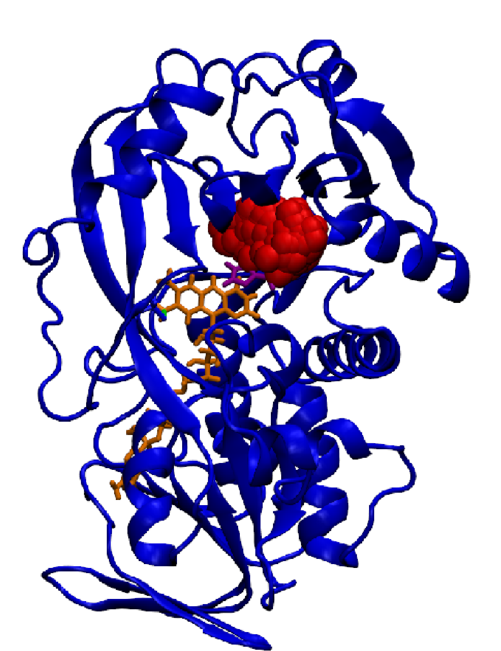
\includegraphics[width=0.45\textwidth]{msox_o2_1}};
\path(nw) +(6,-1) node (image2) [graphics,anchor=north west] {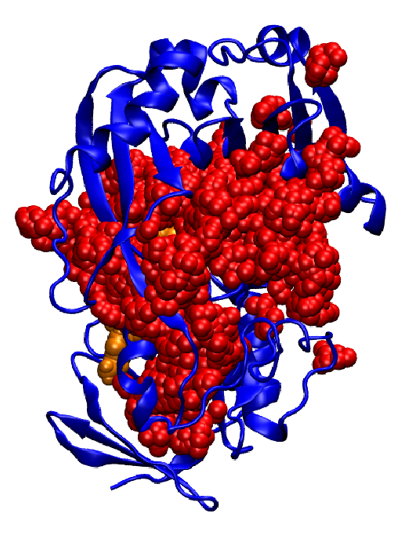
\includegraphics[width=0.45\textwidth]{msox_tamd1}};
\path(nw) +(1.5,-0.5) node (label1) [anchor=north west] {\Large MD};
\path(nw) +(7.5,-0.5) node (label1) [anchor=north west] {\Large TAMD};
\end{tikzpicture}
\end{frame}

\begin{frame}[fragile]{The Method of Single-Sweep Reconstruction}
\begin{tikzpicture}[scaleall=1.0]
\pcuad{\textwidth}{\textheight}
%\showcuad
\path(nw) ++(-0.75,0.15) node(cites)[anchor=north west,text 
width=\textwidth]{{\tiny \textcolor{red!80!black}{
L. Maragliano and E. Vanden-Eijnden, {\it J Chem Phys} {\bf 88}:184110 (2008)
}}};
\path(nw) +(0.0,-1.0) node(text1) [anchor=north west,text width=\textwidth] {
At each $\zb_i$, use \textcolor{green!80!black}{restrained MD} to estimate mean forces $\fb_i$:
\begin{displaymath}
\fb_i = -\left.\frac{\partial F}{\partial \zb}\right|_{\zb_i} \approx \langle \kappa\left[\thetab(\xb)-\zb\right]\rangle_{\zb_i}.
\end{displaymath}
Cast free energy $F(\zb)$ as a superposition of radial Gaussian basis functions $\phi_i$:
\begin{displaymath}
\tilde{F}(\zb) = \sum_i a_i \phi_i (|\zb-\zb_i|;\sigma)
\end{displaymath}
Determine $\tilde{F}$ by finding $\ab,\sigma$ to minimize an error $E(\ab,\sigma)$:
\begin{displaymath}
E(\ab,\sigma) = \sum_i\left|\sum_{i^\prime} a_{i^\prime} \nabla_{\zb}\phi(|\zb_i-\zb_{i^\prime}|;\sigma)+\fb_i\right|^2
\end{displaymath}
};
\end{tikzpicture}
\end{frame}

\begin{frame}[fragile]{Three-Dimensional Free-Energy $F(\zb)$ for O$_{\sf 2}$ in MSOX}
\begin{tikzpicture}[scaleall=1.0]
\pcuad{\textwidth}{\textheight}
%\showcuad
\path(nw) ++(-0.75,0.15) node(cites)[anchor=north west,text 
width=\textwidth]{{\tiny \textcolor{red!80!black}{
A. Bucci and \underline{CFA}, {\it J Chem Theory Comput} {\bf 10}:2668 (2014)
}}};
\path(nw) +(2,-1) node (image1) [graphics,anchor=north west] {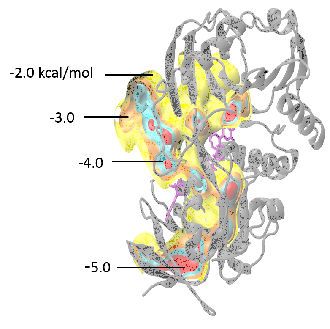
\includegraphics[width=0.6\textwidth]{msox_levels}};
\end{tikzpicture}
\end{frame}

\begin{frame}[fragile]{Milestoning: Temporal Coarse-Graining of MD}
\begin{tikzpicture}[scaleall=1.0]
\pcuad{\textwidth}{\textheight}
%\showcuad
\path(nw) +(-0.75,0.15) node(text)[anchor=north west,text 
width=\textwidth]{{\tiny \textcolor{red!80!black}{A. K. Faradjian and R. Elber {\it J Chem Phys} {\bf 120}:010880 (2004).}}};
\path(nw) +(-0.75,-0.5) node(text1)[anchor=north west,text width=0.5\textwidth]{
Coarsening of a hypothetical infinitely long MD trajectory onto a \textcolor{red}{jump process}};
\path(nw) +(-0.75,-2) node(image1)[anchor=north west]{
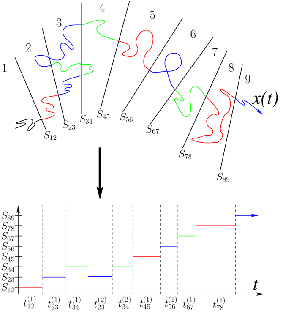
\includegraphics[width=0.5\textwidth]{milestoning1}};
\path(nw) +(5,0) node(text2) [anchor=north west,text width=0.5\textwidth]{
\begin{center}
Coarse-grained kinetics are fully described by a \textcolor{blue}{rate matrix}:
\end{center}
\begin{displaymath}
q_{ik,ij} = \left\{\begin{array}{ll}
\frac{\ds N_{ik,ij}}{\ds R_{ij}} & \mbox{if}\ R_{ij}>0;\\
0 & \mbox{if}\ R_{ij}=0,
\end{array}\right.
\end{displaymath}
where
\begin{align*}
N_{ik,ij} =& \left\{\begin{array}{l}
\mbox{\# of times trajectory}\\
\mbox{collides with $S_{ik}$ after}\\
\mbox{last hitting $S_{ij}$}
\end{array}\right\},\\
R_{ij} = &\left\{\begin{array}{l}
\mbox{total amount of time for}\\
\mbox{which $S_{ij}$ was the last}\\
\mbox{milestone hit}
\end{array}\right\},\\
& = \sum_m t_{ij}^{(m)}.
\end{align*}
};
\end{tikzpicture}
\end{frame}

\begin{frame}[fragile]{Making Milestoning Practical: Transition-Path Theory and \\ Markovian Milestoning in Voronoi Tesselations}
\begin{tikzpicture}[scaleall=1.0]
\pcuad{\textwidth}{\textheight}
%\showcuad
\path(nw) ++(-0.75,0.15) node(text)[anchor=north west,text 
width=\textwidth]{{\tiny \textcolor{red!80!black}{
E. Vanden-Eijnden et al. {\it J Chem Phys} {\bf 130}:194101 (2009).}}};
\path(nw) ++(-0.75,-0.5) node(text2)[anchor=north west,text width=1.1\textwidth]{
Estimate \textcolor{blue}{$\ds q_{ik,ij}$} using MD trajectories confined to Voronoi cells in CV space};
\path(nw) ++(-0.75,-1.5) node(image1)[anchor=north west]{
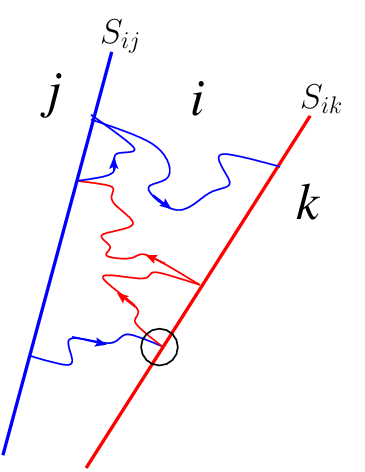
\includegraphics[width=0.4\textwidth]{milestoning2}};
\path(nw) ++(4.25,-1.0) node(text3)[scale=0.7,anchor=north west,text width=0.8\textwidth]{
In each cell $i$, use confined MD of duration $T_i$ to tally:
\begin{enumerate}
\item $N^i_{ik,ij}$,
\item $R^i_{ij}$,\ and,
\item $N^i_{i\rightarrow j}$: \# of transition attemps from $i$ to any neighbor $j$.
\end{enumerate}
Compute apparent transition rate constants:
\begin{displaymath}
k_{i\rightarrow j} = \frac{\ds N^i_{i\rightarrow j}}{\ds T_i}
\end{displaymath}
And enforce equilibrium among all $\Lambda$ cells, so
\begin{displaymath}
\sum_{j=1,j\ne i}^{\Lambda} \pi_j k_{j\rightarrow i} = \pi_i\sum_{j=1;j\ne i}^{\Lambda} k_{i\rightarrow j}\ \ \sum_i\pi_i = 1
\end{displaymath}
providing equilibrium probabilities to be in cell $i$, $\pi_i$.  This allows construction of $q_{ik,ij}$:
\begin{displaymath}
q_{ik,ij} = \frac{\ds \pi_i N^i_{ik,ij}/T_i}{\ds \pi_i R^i_{ij}/T_i + \pi_j R_{ij}^j/T_j}.
\end{displaymath}
};
\end{tikzpicture}
\end{frame}

\begin{frame}[fragile]{Hitting Points on Milestones along O$_{\sf 2}$-Diffusion Pathways in MSOX}
\begin{tikzpicture}[scaleall=1.0]
\pcuad{\textwidth}{\textheight}
%\showcuad
\path(nw) ++(-0.75,0.15) node(text)[anchor=north west,text 
width=\textwidth]{{\tiny \textcolor{red!80!black}{
A. Bucci, T.-Q. Yu, E. Vanden-Eijnden and \underline{CFA} {\it J Chem Theory Comput} {\bf 12}:2964 (2016).}}};
\path(nw) ++(2.5,-0.5) node(image1)[anchor=north west]{
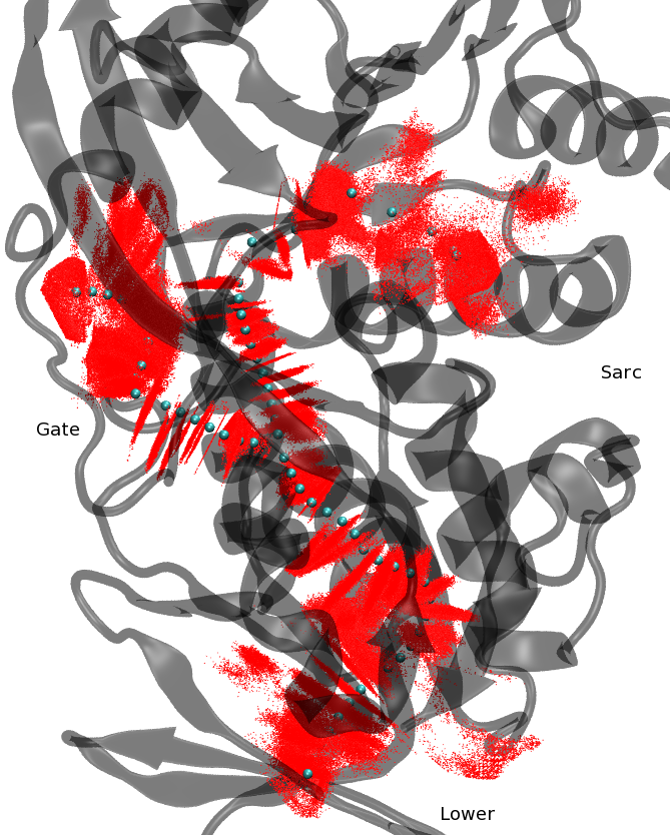
\includegraphics[width=0.5\textwidth]{msox_milestoning}};
\end{tikzpicture}
\end{frame}

\begin{frame}[fragile]{Milestoning Predicts O$_{\sf 2}$ Kinetics Are Sensitive to Substrate}
\begin{tikzpicture}[scaleall=1.0]
\pcuad{\textwidth}{\textheight}
%\showcuad
\path(nw) ++(-0.75,0.15) node(text)[anchor=north west,text 
width=\textwidth]{{\tiny \textcolor{red!80!black}{
A. Bucci, T.-Q. Yu, E. Vanden-Eijnden and \underline{CFA} {\it J Chem Theory Comput} {\bf 12}:2964 (2016).}}};
\path(nw) ++(-0.25,0.5) node(table)
[shape=rectangle,anchor=north west,text width=\textwidth] {
  \begin{table}
%    \caption{Largest cities in the world (source: Wikipedia)}
    \begin{tabular}{llcccc}
      \toprule
       & & $k_1$ & $k_{\sf O_2}$  & $k_{-1}$ & $K_{\rm D}\equiv k_{-1}/k_1$ \\
       & & (M$^{-1}$s$^{-1}$) & (M$^{-1}$s$^{-1}$) & (s$^{-1}$)& (M)\\
      \midrule
      \multirow{2}{*}{Milestoning} & apo & 7.23$\times$10$^{6}$ & --- & 5$\times$10$^7$ & 7.1 \\
      & holo & 2.74$\times$10$^{6}$ & --- & 6$\times$10$^6$ & 2.2 \\
      Experiment* & & --- & 2.8$\times$10$^5$ & --- & ---\\
      \bottomrule
    \end{tabular}
    \raggedright{\Tiny *\textcolor{blue!80!white}{MA Wagner and MS Jorns 
    {\it Biochemistry} {\bf 39}:8825 (2000).}}
  \end{table}
  $\Rightarrow$ Presence of substrate influences O$_{\sf 2}$ entry/exit kinetics.
};
%\path(sw) ++(0,4.0) node(sometext) [anchor=west,shape=rectangle,draw]{
%\begin{align*}
%   (K_D)_{\sf apo} > (K_D)_{\sf holo}  \Rightarrow & 
%   \mbox{presence of substrate \textcolor{green!80!black}{\bf does} influence}\\
% & \mbox{O$_{\sf 2}$ entry/exit kinetics.}\\
% \Rightarrow & \mbox{Support for \textcolor{red}{modified ping-pong}.}
%\end{align*}
%};

\path(sw) ++(0,2.4) node (ErO2) [anchor=west,shape=rectangle] {E$_{\sf R}$ + O$_{\sf 2}$}
          ++(3,0) node (ErsO2) [anchor=west,shape=rectangle] {E$_{\sf R}$*O$_{\sf 2}$}
          ++(3,0) node (Eox) [anchor=west,shape=rectangle] {E$_{\sf O}$};
\path(ErO2) ++(0,1) node (phant1) [anchor=south] {};
\path(Eox) ++(0,1) node (phant2) [anchor=south] {};
%\pgfsetarrowsend{left to}
\draw [white] (ErO2.south east) -- (ErO2.north east) node(labelp1)[pos=0.45]{} node(labelp2)[pos=0.55]{};
\draw [white] (ErsO2.south west) -- (ErsO2.north west) node(labelp3)[pos=0.45]{} node(labelp4)[pos=0.55]{};
\draw [-left to,thick,red] (labelp2) -- (labelp4) node(labelk1)[pos=0.50]{};
\draw [-left to,thick,red] (labelp3) -- (labelp1) node(labelkm1)[pos=0.50]{};
\draw [->,thick,black] (ErsO2.east) -- (Eox.west) node(labelkox)[pos=0.50]{};
\draw [->,thick,green!80!black] (ErO2.north) .. controls (phant1.south) and (phant2.south) .. (Eox.north) node(labelko2)[pos=0.50]{};
\path(labelk1) ++(0,0.22) node (k1) {$k_1$};
\path(labelkm1) ++(0,-0.22) node (kminus1) [shape=rectangle] {$k_{-1}$};
\path(labelkox) ++(0,0.22) node (kox) [shape=rectangle] {$k_{\sf ox}$};
\path(labelko2) ++(0,0.22) node (ko2) [shape=rectangle] {$k_{\sf O_2}$};
\path(ko2) ++(0.75,0) node (textko2) [anchor=west,shape=rectangle] {\small Expt. measures this};
\path(kminus1) ++(0,-1) node (textkm1) [anchor=north,shape=rectangle] {\small Milestoning measures these.};
\draw [->,black,thick] (textko2.west) -- (ko2.east);
\draw [->,black,thick] (textkm1.north) -- (kminus1.south);
\path(Eox) ++(1.5,1) node (textrates) [shape=rectangle,anchor=west] {$\ds k_{\sf O_2} = \frac{k_{\sf ox}}{K_{\rm D}}$}
           ++(-0.5,-0.5) node (labeltext) [shape=rectangle,anchor=north west,text width=0.4\textwidth] {$K_{\rm D}$ may explain observed MPP, {\bf if} $k_{\rm ox}$ is independent of substrate.};
\end{tikzpicture}
\end{frame}

\begin{frame}[fragile]{Mean First-Passage Times along Diffusion Pathways}
\begin{tikzpicture}[scaleall=1.0]
\pcuad{\textwidth}{\textheight}
%\showcuad
\path(nw) ++(-0.75,0.15) node(text)[anchor=north west,text 
width=\textwidth]{{\tiny \textcolor{red!80!black}{
A. Bucci, T.-Q. Yu, E. Vanden-Eijnden and \underline{CFA} {\it J Chem Theory Comput} {\bf 12}:2964 (2016).}}};
\path(c2) ++(0,-1) node(aas)[shape=rectangle] {Active} 
          ++(0,2.0) node(aMidLys) [shape=rectangle] {Mid-Lys}
          ++(-2.4,-2.0) node(aGateLys) [shape=rectangle] {Gate-Lys}
          ++(4.6,0) node(aSarc) [shape=rectangle] {Sarc}
          ++(-3.5,1.5) node(ApoLabel) [shape=rectangle,draw,thick,anchor=south] {{\it Apo}}
          ++(0,-2.5) node(conclabel) [shape=rectangle,draw,blue!80!black,anchor=north west] {\textcolor{blue}{[O$_{\sf 2}$] = 0.26 mM}};
\path(c3) ++(0,0) node(has)[shape=rectangle] {Active} 
          ++(-2.4,0) node(hGateLys) [shape=rectangle] {Gate-Lys}
          ++(4.6,0) node(hSarc) [shape=rectangle] {Sarc}
          ++(-3.5,1) node(HoloLable) [shape=rectangle,draw,thick,anchor=south] {{\it Holo}};
\draw[thick,red,transform canvas={yshift=-0.3ex},-right to] (aGateLys) -- node[below]{700\ $\mu$s} (aas);
\draw[thick,green!80!black,transform canvas={yshift=0.3ex},-right to] (aas) -- node[above]{0.1\ $\mu$s} (aGateLys);
\draw[thick,green!80!black,transform canvas={yshift=0.3ex},-left to] (aas) -- node[above]{0.1\ $\mu$s} (aSarc);
\draw[thick,red,transform canvas={yshift=-0.3ex},-left to] (aSarc) -- node[below]{900\ $\mu$s} (aas);

\draw[thick,red,transform canvas={xshift=-0.3ex},-right to] (aMidLys) -- node[left]{200\ $\mu$s} (aas);
\draw[thick,green!80!black,transform canvas={xshift=0.3ex},-right to] (aas) -- node[right]{0.03\ $\mu$s} (aMidLys);

\draw[thick,red,transform canvas={yshift=-0.3ex},-right to] (hGateLys) -- node[below]{7000\ $\mu$s} (has);
\draw[thick,green!80!black,transform canvas={yshift=0.3ex},-right to] (has) -- node[above]{3\ $\mu$s} (hGateLys);
\draw[thick,green!80!black,transform canvas={yshift=0.3ex},-left to] (has) -- node[above]{0.2\ $\mu$s} (hSarc);
\draw[thick,red,transform canvas={yshift=-0.3ex},-left to] (hSarc) -- node[below]{500\ $\mu$s} (has);
\path(np) ++(0,-2.5) node(bigtext) [shape=rectangle,anchor=north west,text width=0.5\textwidth] {
Substrate binding:
\begin{itemize}
\item effectively shuts down entry through all pathways {\em except} one (``Sarc'').
\item slows exit through all pathways.
\end{itemize}};

%\draw [white] (aas.south west) -- (aas.north west) node(aasll) [pos=0.45]{} node(aasul) [pos=0.55]{};
%\draw [white] (aas.south east) -- (aas.north east) node(aaslr) [pos=0.45]{} node(aasur) [pos=0.55]{};
%\draw [white] (aGateLys.south east) -- (aGateLys.north east) node(agllr) [pos=0.45]{} node(aglur) [pos=0.55]{};
%\draw [white] (aSarc.south west) -- (aSarc.north west) node(asll) [pos=0.45]{} node(asul) [pos=0.55]{};
%\draw [-left to,thick,red] (aglur) -- (aasul);
%\draw [-left to,thick,red] (aasll) -- (agllr);
%\draw [-left to,thick,red] (aasur) -- (asul);
%\draw [-left to,thick,red] (asll) -- (aaslr);
\end{tikzpicture}
\end{frame}

\begin{frame}[fragile]{Independent Predictions of Substrate-Induced O$_{\sf 2}$ Slowdown}
\begin{tikzpicture}[scaleall=1.0]
\pcuad{\textwidth}{\textheight}
%\showcuad
\path(nw) ++(-0.75,0.15) node(text)[anchor=north west,text 
width=\textwidth]{{\tiny \textcolor{red!80!black}{
A. Bucci, T.-Q. Yu, E. Vanden-Eijnden and \underline{CFA} {\it J Chem Theory Comput} {\bf 12}:2964 (2016).}}};
\path(np) ++(-5.5,-0.50) node(image1) [graphics,anchor=north west] {
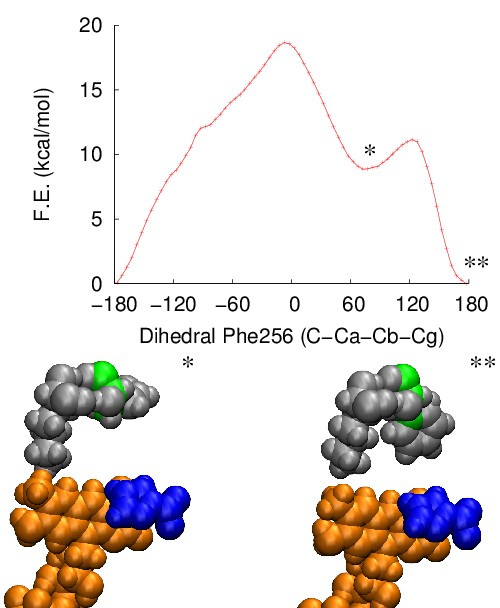
\includegraphics[width=0.5\textwidth]{msox_ph256_gate}}
+(0,-6.5) node(text1) [anchor=north west,text width=0.5\textwidth] {Substrate induces closure of Phe256 ``gate''.}
++(6.0,-1) node(image2) [graphics,anchor=north west] {
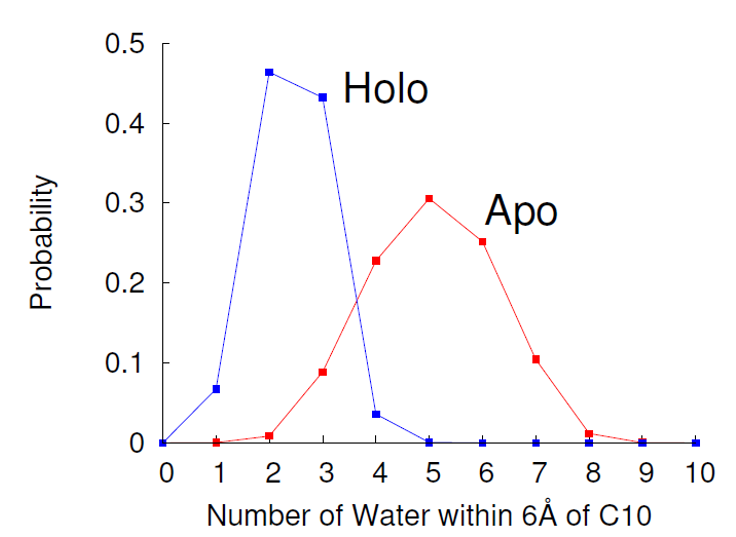
\includegraphics[width=0.5\textwidth]{msox_water}}
+(0,-4) node(text2) [anchor=north west,text width=0.5\textwidth] {Substrate pushes waters out of active site.};
\end{tikzpicture}
\end{frame}
\section{Summary}

\begin{frame}[fragile]{Summary}
\begin{itemize}
\item OTFP combines enhanced sampling and free-energy-profile generation to provide deeper understanding of biomolecular mechanisms
\item We recapitulate water-mediated ``knock-on'' transport of multiple K$^+$ ions in Kv1.2, but also predict reduced barriers for dry transport
\item Demonstrated Markovian milestoning along minimum free-energy pathways to estimate entry and exit rates of O$_{\sf 2}$ in MSOX
\item MSOX: Simulations agree with experiment that modified ping-pong mechanism is more likely than ping-pong because substrate influences O$_{\sf 2}$
entry and exit kinetics
\item MSOX: Substrate-induced gatekeeper closing and active-site desolvation likely underly the substrates effect on O$_{\sf 2}$.
%\item Demonstrated a new algorithm for ISRE based on Gillespie's algorithm (like Kinetic Monte-Carlo)i that outperforms RE in a protein-folding calculation
%\item ``Discovered'' new stable, non-native folded state for the protein-G $\beta$ hairpin
\end{itemize}
\end{frame}

\begin{frame}[fragile]{Acknowledgments}
\begin{tikzpicture}[scaleall=1.0]
\pcuad{\textwidth}{\textheight}
%\showcuad
\path(nw) ++(-0.5,0.0) node(text1) [anchor=north west,text width=1.1\textwidth,execute at begin node=\setlength{\baselineskip}{1em}]{
\small Steven GOSSERT $\bullet$ Natasha VERGARA $\bullet$
Ming HUANG $\bullet$ Dr. Salman ZARRINI $\bullet$ Dr. Gourav SHRIVASTAV $\bullet$ Dr. Mohammadjavad MOHAMMADI 
}
 ++(0.0,-1.25) node(ack) [graphics,anchor=north west]{
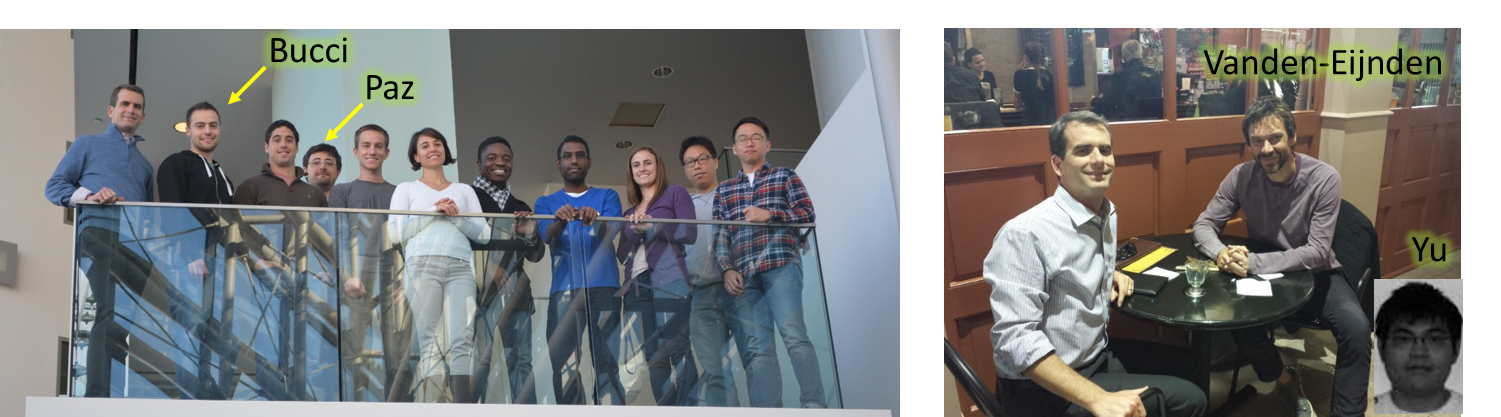
\includegraphics[width=1.1\textwidth]{ack}}
++(0.0,-3.25) node(text2) [anchor=north west,text width=1.1\textwidth,execute at begin node=\setlength{\baselineskip}{0.75em}]{
\tiny \textcolor{orange!80!black}{\it Alumni:} Dr. Yelena SLIOZBERG (ARL) $\bullet$
Prof. Ehsan JABBARZADEH (USC) $\bullet$
Prof. Harish VASHISTH (UNH) $\bullet$
Dr. Spencer STOBER (ExxonMobil) $\bullet$
Dr. Ali EMILEH (BASF Enzymes) $\bullet$
Dr. Vamshi GANGUPOMU (TVS) $\bullet$ 
Dr. Michelle BAKER (J\&J) $\bullet$
{\bf Dr. Anthony BUCCI} (West Pharma) $\bullet$
Dr. Ryan GORDON (OSISoft) $\bullet$
Dr. Arun SRIKANTH (Bath) $\bullet$
Dr. Jasmine GARDNER (Uppsala) $\bullet$
{\bf Prof. S. Alexis PAZ} (NUCordoba in Argentina) $\bullet$
Dr. Samba Somisetti $\bullet$
Dr. Changwoon JANG (Nagoya) $\bullet$
Dr. Mauro LAPELOSA $\bullet$
Dr. Debashish MUKHERJI (MPI-P) $\bullet$
Dr. Francesca MORACA (Schrodinger, Inc.)}
++(0.0,-1.25) node(text2) [anchor=north west,text width=1.1\textwidth,execute at begin node=\setlength{\baselineskip}{1em}]{
\small \textcolor{blue}{\em Collaborators:}  {\bf Tang-Qing YU} $\bullet$ {\bf Eric VANDEN-EIJNDEN (NYU)}
$\bullet$ Irwin CHAIKEN (DUCOM) $\bullet$ Amos SMITH III (UPenn Chem)}
++(0.0,-1) node(text2) [anchor=north west,text width=\textwidth,execute at begin node=\setlength{\baselineskip}{1em}]{
\textcolor{green!80!black}{Funding (this talk):} NIH R01GM100472, NSF DMR1207389\\   \textcolor{red}{Computing:}  XSEDE, Drexel Proteus};
\end{tikzpicture}
\end{frame}


\end{document}
